\chapter{Kravspecifikation}

Følgende er en beskrivelse af de aktuelle krav stillet til projektet, i samarbejde mellem Rambøll og projektgruppen. De er alle opstillet som user stories. User stories er korte beskrivelser af funktionalitet, som står på en fast form. De er let læselige og har værdi for både personer direkte involveret i projektet og udefrakommende, som skal opnå en idé om kravene til projektet. 

\section{Aktør kontekst diagram}\label{sec:Aktor}
	På figur \ref{fig:AktorKontekst} ses aktør/kontekst diagrammet for Rambøll Tilsyn. 
\begin{figure}[H]
	\centering
	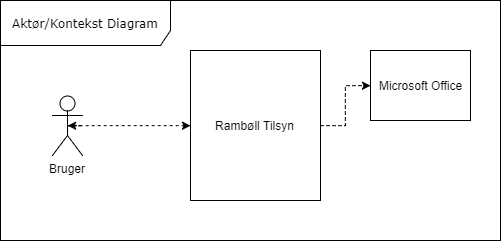
\includegraphics[width=0.6\linewidth]{FunktionelleKrav/AktorDiagram}
	\caption{Aktør/kontekst diagram for Rambøll Tilsyn}
	\label{fig:AktorKontekst}
\end{figure}
Det ses at systemet har følgende aktører:
\begin{itemize}
	\item Primær aktør: Bruger
	\item Sekundær aktør: Microsoft Office \\
\end{itemize}

Brugern kan benytte systemet Rambøll Tilsyn. Systemet bruger Microsoft Office til at eksportere information fra applikationen til Excel.

\clearpage

\section{Funktionelle Krav} \label{sec:UserStories}
I følgende afsnit vil der være en beskrivelse af de funktionlle krav for Rambøll Tilsyn.

\subsection{User stories diagram}
På figur \ref{fig:Userstoriediagram} ses User Stories diagrammet for systemet. Systemet har 19 User Stories, som tilsammen beskriver funktionaliteten for systemet. \\

\begin{figure}[H]
	\centering
	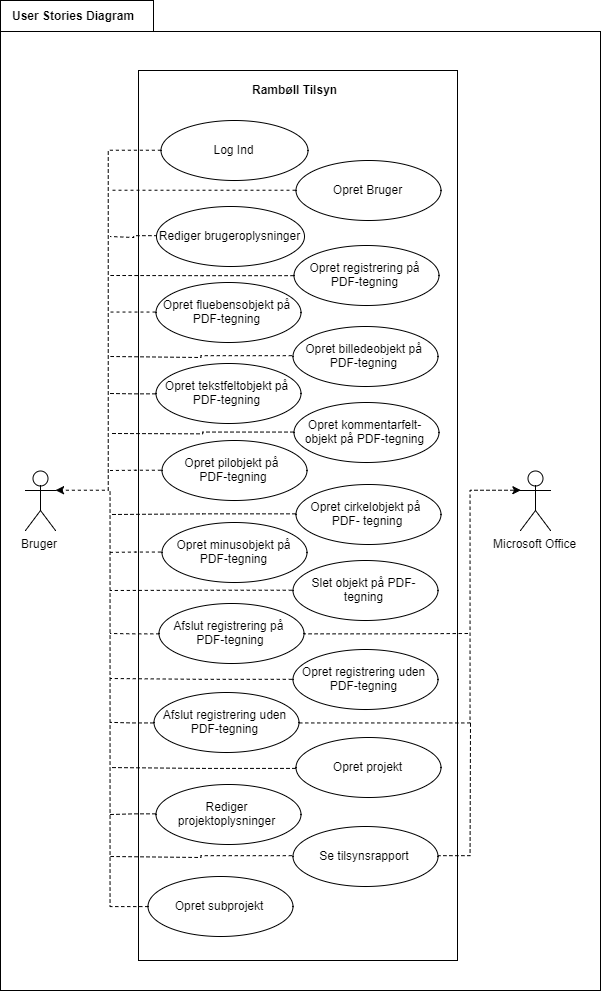
\includegraphics[width=0.6\linewidth]{FunktionelleKrav/UserStorieDiagram}
	\caption{User stories diagram for Rambøll Tilsyns App}
	\label{fig:Userstoriediagram}
\end{figure}

Aktørene fra aktør kontekst diagrammet figur \ref{fig:AktorKontekst} går igen i User Stories diagrammet. Det er brugeren som primær bruger, der benytter systemet. Mens at systemet benytter den sekundære aktør Microsoft Office.

\clearpage

\subsection{User stories beskrevet med Gherkin}
Til beskrivelse af user stories er Gherkin-syntaksen\cite{Gherkin} valgt, hvor stories 
kan skrives på et flydende sprog, mens de er testbare. Gherkin-syntaksen er et Business-Readable Domain  
Specific Language. En fordel ved anvendelsen af syntaksen er, at den opstiller kravene, så de er testbare, hvilket medfører, at kravene for test af features er skrevet i user stories.
Gherkin anvender nøgleord i det flg. afsnit 
markeret med blåt,  som hver især har en funktion i beskrivelsen af hver 
user story. Dette vil blive beskrevet i følgende afsnit.  \vspace{0.2 cm}\\
Første del i Gherkin modellen er en egenskab, som indeholder en beskrivelse af forretningsdomænet. 
Formatet i	dette afsnit vælges frit. Det anbefales, at man anvender et 
system, hvor der som minimum svares på, hvilke aktører der har et behov, hvad 
behovet består af og hvorfor aktører har dette behov. En tre trins user 
story opfylder dette krav og opstilles med tre 
sætninger. Første sætning svarer på, hvilken aktør eller aktør(er) der har
behovet. Dernæst svarer man på, hvad det konkret er at aktøreren ønsker at 
opnå. Den tredje sætning beskriver aktørens motivation for at anvende 
funktionaliteten. \\
Samtlige nøgleord beskrives nedenfor:

\large{\textbf{Givet}}\\
Disse trin definerer tilstande og datastrukturer, som anvendes i de 
efterfølgende trin og scenarier.

\large{\textbf{Når}}\\
Disse trin beskriver handlinger, som ændrer Scenariets tilstand. Dette kan 
være handlinger	foretaget af aktøreren og/eller systemet.

\large{\textbf{Så}}\\
Disse trin definerer udfaldet af forudgående handlinger i et givet 
scenarie. Alle scenarier skal afsluttes ved at definere det forventede 
udfald i et eller flere Så trin.

\large{\textbf{Scenarier}}\\
Scenarier er samlinger af trin, som definerer de funktionelle krav til 
forløb. Første scenarie i en egenskab dækker hovedfunktionaliteten. De 
efterfølgende scenarier dækker fejlhåndteringer og alternative scenarier.

\large{\textbf{Baggrund}}\\
Baggrund er en særlig type scenarie, som udføres inden hvert af de 
efterfølgende scenarier	i egenskaben. Systemets tilstand og preconditions 
beskrives under overskriften Baggrund efterfulgt af et kolon og 
linjeskift. Herefter listes alle de data, tilstande og handlinger, som udgør 
systemets tilstand inden samtlige af de efterfølgende Scenarier kan	udføres.


\subsection{Log ind (CRS-1)} \label{sec:USLogInd}
\textbf{\textsc{\textcolor{RoyalBlue} {Egenskab:} Log-in på applikationen}} \\
Som bruger\\
Ønsker jeg at kunne logge ind på applikationen\\
For at kunne benytte applikationen\\ \\

\textbf{\textsc{\color{RoyalBlue}Baggrund:}}\\
\textcolor{RoyalBlue}{Givet} følgende eksisterende profil\\
\begin{tabular}{| l | l | l | l |}
	\textbf{fornavn} & \textbf{efternavn} & \textbf{e-mail} & \textbf{kode} \\
	Ao & Testbruger & test@ramboell.dk & Test123\\
\end{tabular}
\newline \newline
\textcolor{RoyalBlue}{Og} Ao er ikke allerede logget ind i systemet\\
\textcolor{RoyalBlue}{Og} han har navigeret til applikationens log-in side\\

\textbf{\textsc{\textcolor{RoyalBlue}{Scenarie:}} Log ind med korrekte oplysninger}\\
\textcolor{RoyalBlue}{Når} Ao indtaster sin mail og kode i de korrekte tekstfelter\\
\textcolor{RoyalBlue}{Og} han trykker på log-in knappen\\
\textcolor{RoyalBlue}{Så} navigeres han til applikationens forside\\

\textbf{\textsc{\textcolor{RoyalBlue}{Scenarie:}} Log ind med forkerte oplysninger} \\
\textcolor{RoyalBlue}{Når} Ao indtaster følgende oplysninger:\\
\begin{tabular}{| l | l |}
	\textbf{e-mail} & \textbf{kode}\\
	Ao@mail.dk & 123\\
\end{tabular}


\textcolor{RoyalBlue}{Og} han trykker på log-in knappen\\
\textcolor{RoyalBlue}{Så} informeres han om, at der er indtastet forkerte oplysninger\\
\textcolor{RoyalBlue}{Og} han bliver på log-in siden \\

\subsection{Opret bruger (CRS-2)} \label{sec:USOpretBruger}
\textbf{\textsc{\textcolor{RoyalBlue}{Egenskab:} Opret bruger}} \\
Som bruger\\
Ønsker jeg at kunne oprette en bruger på applikationen\\
For at kunne give en anden bruger adgang til systemet \\

\textcolor{RoyalBlue}{\textbf{\textsc{Baggrund:}}}\\
\textcolor{RoyalBlue}{Givet} at brugeren Rasmus er logget ind \\
\textcolor{RoyalBlue}{Og} han vil oprette en bruger med følgende oplysninger:\\
\begin{tabular}{| l | l |}
	\textbf{e-mail} & \textbf{kode} \\
	jakob@ramboell.dk & solskin\\
\end{tabular}
\newline \newline
\textcolor{RoyalBlue}{Og} han er navigeret til opret bruger siden for at oprette brugere  \\

\textbf{\textsc{\textcolor{RoyalBlue}{Scenarie:}} Opret bruger}\\
\textcolor{RoyalBlue}{Når} Rasmus indtaster mail, kode, telefonnummer, 
fornavn og efternavn \\
\textcolor{RoyalBlue}{Og} trykker på opret bruger-knappen\\
\textcolor{RoyalBlue}{Så} oprettes den nye bruger\\
\textcolor{RoyalBlue}{Og} den nye bruger kan logge ind\\

\subsection{Rediger brugeroplysninger (CRS-3)} \label{sec:USRedigerBruger}
\textbf{\textsc{\textcolor{RoyalBlue}{Egenskab:} Rediger brugeroplysninger}}\\
Som bruger\\
Ønsker jeg at kunne ændre brugeroplysninger\\
For at have aktuelle oplysninger

\textsc{\textcolor{RoyalBlue}{\textbf{Baggrund:}}}\\
\textcolor{RoyalBlue}{Givet} at Niels er logget ind\\
\textcolor{RoyalBlue}{Og} han har følgende nuværende oplysninger:\\
\begin{tabular}{| l | l | l |}
	\textbf{fornavn} & \textbf{efternavn} & \textbf{kodeord} \\
	Niels & Testbruger & paris \\
\end{tabular}
\newline \newline
\textcolor{RoyalBlue}{Og} at han vil ændre indstillingerne til følgende:\\
\begin{tabular}{| l | l | l | l |}
	\textbf{fornavn} & \textbf{efternavn} & \textbf{kodeord} \\
	Niels & TestTest & london \\
\end{tabular}
\newline \newline
\textcolor{RoyalBlue}{Og} at han er navigeret til \emph{rediger bruger siden} \\

\textbf{\textsc{\textcolor{RoyalBlue}{Scenarie:}} Rediger kode}\\
\textcolor{RoyalBlue}{Når} Niels indtaster paris i kodefeltet Gammel adgangskode\\
\textcolor{RoyalBlue}{Og} han skriver london i Ny adgangskode og Bekræft ny adgangskode\\
\textcolor{RoyalBlue}{Og} han trykker på gem oplysninger\\
\textcolor{RoyalBlue}{Så} gemmes oplysningerne\\
\textcolor{RoyalBlue}{Og} han informeres om at ændringerne er gemt

\textbf{\textsc{\textcolor{RoyalBlue}{Scenarie:}} Rediger for- og efternavn}\\
\textcolor{RoyalBlue}{Når} Niels indtaster nyt for- og efternavn i de korrekte tekstfelter\\
\textcolor{RoyalBlue}{Og} han trykker på ok\\
\textcolor{RoyalBlue}{Så} gemmes oplysningerne\\
\textcolor{RoyalBlue}{Og} han kan se at ændringerne er gemt \\

\textbf{\textsc{\textcolor{RoyalBlue}{Scenarie:}} Rediger telefonnummer}\\
\textcolor{RoyalBlue}{Når} Niels indtaster 87654321 i det korrekte tekstfelt\\
\textcolor{RoyalBlue}{Og} han trykker på ok\\
\textcolor{RoyalBlue}{Så} gemmes oplysningerne\\
\textcolor{RoyalBlue}{Og} han kan se at ændringerne er gemt \\

\subsection{Opret en registrering på PDF-tegning (CRS-4)} \label{sec:USOpretRegPåPDF}
\textbf{\textsc{\textcolor{RoyalBlue}{Egenskab:} Opret en registrering på PDF-tegning}}\\
Som bruger\\
Ønsker jeg at kunne oprette en registrering på en PDF\\
For kunne lave en registrering på et givent projekts pdf tegning \\ \\

\textsc{\textcolor{RoyalBlue}{\textbf{Baggrund:}}}\\
\textcolor{RoyalBlue}{Givet} at Søren er logget ind\\
\textcolor{RoyalBlue}{Og} han har følgende nuværende oplysninger:\\
\begin{tabular}{| l | l |}
	\textbf{fornavn} & \textbf{rolle} \\
	Søren & Bruger\\
\end{tabular}

\textbf{\textsc{\textcolor{RoyalBlue}{Scenarie:}} Opret en registrering på PDF-tegning}\\
\textcolor{RoyalBlue}{Når} Søren vælger Opret registrering på PDF-tegning\\
\textcolor{RoyalBlue}{Så}  navigeres han videre til registreringssiden\\
\textcolor{RoyalBlue}{Så}  har han mulighed for at indsætte objekter på PDF-tegningen, som en del af sin registrering\\
\textcolor{RoyalBlue}{Når} han er færdig med at registrer kan han vælge afslut \\
\textcolor{RoyalBlue}{Så}  navigeres hans videre til fejl rapporten for alle objekter oprettet på projektet \\

\subsection{Opret fluebensobjekt på PDF-tegning (CRS-5)} \label{sec:USOpretFlueben}
\textbf{\textsc{\textcolor{RoyalBlue}{Egenskab:} Opret fluebensobjekt på PDF-tegning}}\\
Som bruger\\
Ønsker jeg at kunne oprette et fluebensobjekt på en PDF-tegning\\
For at kunne opdatere min registrering på et givent projekt \\

\textsc{\textcolor{RoyalBlue}{\textbf{Baggrund:}}}\\
\textcolor{RoyalBlue}{Givet} at Søren er logget ind\\
\textcolor{RoyalBlue}{Og} han har følgende nuværende oplysninger:\\
\begin{tabular}{| l | l |}
	\textbf{fornavn} & \textbf{rolle} \\
	Søren & Bruger\\
\end{tabular}

\textbf{\textsc{\textcolor{RoyalBlue}{Scenarie:}} Opret fluebensobjekt på PDF--tegning}\\
\textcolor{RoyalBlue}{Når} Søren trykker på fluebensobjektet\\
\textcolor{RoyalBlue}{Så}  får han valgmuligheden om, hvilken farve han ønsker fluebenet skal have\\
\textcolor{RoyalBlue}{Så}  har han mulighed for at sætte objektet et sted på PDF-tegningen\\
\textcolor{RoyalBlue}{Når} han har placeret fluebensobjektet, kan han oprette et nyt objekt, slette et objekt eller vælge at afslutte \\

\subsection{Opret billedeobjekt på PDF-tegning (CRS-6)} \label{sec:USOpretBillede}
\textbf{\textsc{\textcolor{RoyalBlue}{Egenskab:} Opret billedeobjekt på PDF-tegning}}\\
Som bruger\\
Ønsker jeg at kunne oprette et billedeobjekt på en PDF\\
For at kunne opdatere min registrering på et givent projekt \\

\textsc{\textcolor{RoyalBlue}{\textbf{Baggrund:}}}\\
\textcolor{RoyalBlue}{Givet} at Jan er logget ind\\
\textcolor{RoyalBlue}{Og} han har følgende nuværende oplysninger:\\
\begin{tabular}{| l | l |}
	\textbf{fornavn} & \textbf{rolle} \\
	Jan & Bruger\\
\end{tabular}

\textbf{\textsc{\textcolor{RoyalBlue}{Scenarie:}} Opret billedeobjekt på PDF-tegning}\\
\textcolor{RoyalBlue}{Når} Jan trykker på billede objektet\\
\textcolor{RoyalBlue}{Så}  har han mulighed for at sætte objektet et sted på PDF-tegningen\\
\textcolor{RoyalBlue}{Så}  åbnes hans kamera og han kan nu tilføje et billede, og derefter en billede tekst\\
\textcolor{RoyalBlue}{Når} han har placeret billedeobjektet, kan han oprette et nyt objekt, slette et objekt eller vælge at afslutte \\

\subsection{Opret tekstfeltobjekt på PDF-tegning (CRS-7)} \label{sec:USOpretTekstfelt}
\textbf{\textsc{\textcolor{RoyalBlue}{Egenskab:} Opret tekstfeltobjekt på PDF-tegning}}\\
Som bruger\\
Ønsker jeg at kunne oprette et tekstfeltobjekt på en PDF\\
For at kunne opdatere min registrering på et givent projekt \\

\textsc{\textcolor{RoyalBlue}{\textbf{Baggrund:}}}\\
\textcolor{RoyalBlue}{Givet} at Jan er logget ind\\
\textcolor{RoyalBlue}{Og} han har følgende nuværende oplysninger:\\
\begin{tabular}{| l | l |}
	\textbf{fornavn} & \textbf{rolle} \\
	Jan & Bruger\\
\end{tabular}

\textbf{\textsc{\textcolor{RoyalBlue}{Scenarie:}} Opret tekstfeltobjekt på PDF-tegning}\\
\textcolor{RoyalBlue}{Når} Jan trykker på tekstfeltobjektet\\
\textcolor{RoyalBlue}{Så}  har han mulighed for at sætte objektet et sted på PDF-tegningen\\
\textcolor{RoyalBlue}{Så}  har han mulighed for at skrive en tekst, som ligger som et objekt han kan åbne og læse teksten\\
\textcolor{RoyalBlue}{Når} han har placeret teskstfeltobjektet, kan han oprette et nyt objekt, slette et objekt eller vælge at afslutte \\

\subsection{Opret kommentarfeltobjekt på PDF-tegning (CRS-8)} \label{sec:USOpretKommentarfelt}
\textbf{\textsc{\textcolor{RoyalBlue}{Egenskab:} Opret kommentarfeltobjekt på PDF-tegning}}\\
Som bruger\\
Ønsker jeg at kunne oprette et kommentarfeltobjekt på en PDF\\
For at kunne opdatere min registrering på et givent projekt \\

\textsc{\textcolor{RoyalBlue}{\textbf{Baggrund:}}}\\
\textcolor{RoyalBlue}{Givet} at Morten er logget ind\\
\textcolor{RoyalBlue}{Og} han har følgende nuværende oplysninger:\\
\begin{tabular}{| l | l |}
	\textbf{fornavn} & \textbf{rolle} \\
	Morten & Bruger\\
\end{tabular}

\clearpage

\textbf{\textsc{\textcolor{RoyalBlue}{Scenarie:}} Opret kommentarfeltobjekt på PDF-tegning}\\
\textcolor{RoyalBlue}{Når} Morten trykker på kommentarfeltobjektet\\
\textcolor{RoyalBlue}{Så}  har han mulighed for at sætte objektet et sted på PDF-tegningen\\
\textcolor{RoyalBlue}{Så}  har han mulighed for at skrive en tekst, som vises på PDF-tegningen\\
\textcolor{RoyalBlue}{Når} han har placeret kommentarfeltobjekt, kan han oprette et nyt objekt, slette et objekt eller vælge at afslutte \\

\subsection{Opret pilobjekt på PDF-tegning (CRS-9)} \label{sec:USOpretPilObjekt}
\textbf{\textsc{\textcolor{RoyalBlue}{Egenskab:} Opret pilobjekt på PDF-tegning}}\\
Som bruger\\
Ønsker jeg at kunne oprette et pilobjekt på en PDF\\
For at kunne opdatere min registrering på et givent projekt \\

\textsc{\textcolor{RoyalBlue}{\textbf{Baggrund:}}}\\
\textcolor{RoyalBlue}{Givet} at Morten er logget ind\\
\textcolor{RoyalBlue}{Og} han har følgende nuværende oplysninger:\\
\begin{tabular}{| l | l |}
	\textbf{fornavn} & \textbf{rolle} \\
	Morten & Bruger\\
\end{tabular}

\textbf{\textsc{\textcolor{RoyalBlue}{Scenarie:}} Opret pilobjekt på PDF-tegning}\\
\textcolor{RoyalBlue}{Når} Morten trykker på pilobjektet\\
\textcolor{RoyalBlue}{Så}  har han mulighed for at sætte objektet et sted på PDF-tegningen\\
\textcolor{RoyalBlue}{Så}  har han mulighed for at trække i pilen så den passer i længde og retning\\
\textcolor{RoyalBlue}{Når} han har placeret pilobjektet, kan han oprette et nyt objekt, slette et objekt eller vælge at afslutte \\

\subsection{Opret cirkelobjekt på PDF-tegning (CRS-10)} \label{sec:USOpretCirkelObjekt}
\textbf{\textsc{\textcolor{RoyalBlue}{Egenskab:} Opret cirkelobjekt på PDF-tegning}}\\
Som bruger\\
Ønsker jeg at kunne oprette et cirkelobjekt på en PDF\\
For at kunne opdatere min registrering på et givent projekt \\

\textsc{\textcolor{RoyalBlue}{\textbf{Baggrund:}}}\\
\textcolor{RoyalBlue}{Givet} at Morten er logget ind\\
\textcolor{RoyalBlue}{Og} han har følgende nuværende oplysninger:\\
\begin{tabular}{| l | l |}
	\textbf{fornavn} & \textbf{rolle} \\
	Morten & Bruger\\
\end{tabular}

\textbf{\textsc{\textcolor{RoyalBlue}{Scenarie:}} Opret cirkelobjekt på PDF-tegning}\\
\textcolor{RoyalBlue}{Når} Morten trykker på cirkelobjektet\\
\textcolor{RoyalBlue}{Så}  har han mulighed for at sætte objektet et sted på PDF-tegningen\\
\textcolor{RoyalBlue}{Så}  har han mulighed for at trække i cirklen så den passer i radius\\
\textcolor{RoyalBlue}{Når} han har placeret cirkelobjektet, kan han oprette et nyt objekt, slette et objekt eller vælge at afslutte \\

\subsection{Opret minusobjekt på PDF-tegning (CRS-11)} \label{sec:USOpretMinusObjekt}
\textbf{\textsc{\textcolor{RoyalBlue}{Egenskab:} Opret minusobjekt på PDF-tegning}}\\
Som bruger\\
Ønsker jeg at kunne oprette et minusobjekt på en PDF\\
For at kunne opdatere min registrering på et givent projekt \\

\textsc{\textcolor{RoyalBlue}{\textbf{Baggrund:}}}\\
\textcolor{RoyalBlue}{Givet} at Lars er logget ind\\
\textcolor{RoyalBlue}{Og} han har følgende nuværende oplysninger:\\
\begin{tabular}{| l | l |}
	\textbf{fornavn} & \textbf{rolle} \\
	Lars & Bruger\\
\end{tabular}

\textbf{\textsc{\textcolor{RoyalBlue}{Scenarie:}} Opret minusobjekt på PDF-tegning}\\
\textcolor{RoyalBlue}{Når} Lars trykker på minusobjektet\\
\textcolor{RoyalBlue}{Så}  har han mulighed for at sætte objektet et sted på PDF-tegningen \\
\textcolor{RoyalBlue}{Når} han har placeret minusobjektet, kan han oprette et nyt objekt, slette et objekt eller vælge at afslutte \\

\subsection{Slet objekt på PDF-tegning (CRS-12)} \label{sec:USSletObjekt}
\textbf{\textsc{\textcolor{RoyalBlue}{Egenskab:} Slet objekt på PDF-tegning}}\\
Som bruger\\
Ønsker jeg at kunne slette et objekt på en PDF\\
For at kunne opdatere min registrering på et givent projekt \\

\textsc{\textcolor{RoyalBlue}{\textbf{Baggrund:}}}\\
\textcolor{RoyalBlue}{Givet} at Lars er logget ind\\
\textcolor{RoyalBlue}{Og} han har følgende nuværende oplysninger:\\
\begin{tabular}{| l | l |}
	\textbf{fornavn} & \textbf{rolle} \\
	Lars & Bruger\\
\end{tabular}

\textbf{\textsc{\textcolor{RoyalBlue}{Scenarie:}} Slet objekt på PDF-tegning}\\
\textcolor{RoyalBlue}{Når} Lars trykker på viskelæder objektet\\
\textcolor{RoyalBlue}{Så}  har han mulighed for slette et objektet på PDF-tegningen\\
\textcolor{RoyalBlue}{Når} han trykker på objektet, slettes dette. Han kun nu oprette et nyt objekt, slette et objekt eller vælge at afslutte \\

\clearpage

\subsection{Afslut registrering på PDF-tegning (CRS-13)} \label{sec:USAfslutRegPåPDF}
\textbf{\textsc{\textcolor{RoyalBlue}{Egenskab:} Afslut registrering på PDF-tegning}}\\
Som bruger\\
Ønsker jeg at kunne afslutte min registrering\\
For at kunne afslutte en registrering på et projekt\\

\textsc{\textcolor{RoyalBlue}{\textbf{Baggrund:}}}\\
\textcolor{RoyalBlue}{Givet} at Jakob er logget ind\\
\textcolor{RoyalBlue}{Og} han har følgende nuværende oplysninger:\\
\begin{tabular}{| l | l |}
	\textbf{fornavn} & \textbf{rolle} \\
	Jakob & Bruger\\
\end{tabular}
\newline

\textbf{\textsc{\textcolor{RoyalBlue}{Scenarie:}} Afslut registrering på PDF-tegning}\\
\textcolor{RoyalBlue}{Når} Jakob trykker på submenu ikonet\\
\textcolor{RoyalBlue}{Så}  har han mulighed for afslut og eksporter\\
\textcolor{RoyalBlue}{Så}  navigeres han til sin mail, hvor en ny mail åbner med en vedhæftet excel fil\\

\subsection{Opret en registrering uden PDF-tegning (CRS-14)} \label{sec:USOpretRegUdenPDF}
\textbf{\textsc{\textcolor{RoyalBlue}{Egenskab:} Opret en registrering uden PDF-tegning}}\\
Som bruger\\
Ønsker jeg at kunne oprette en registrering uden en PDF\\
For kunne lave en registrering på et givent projekt\\

\textsc{\textcolor{RoyalBlue}{\textbf{Baggrund:}}}\\
\textcolor{RoyalBlue}{Givet} at Dan er logget ind\\
\textcolor{RoyalBlue}{Og} han har følgende nuværende oplysninger:\\
\begin{tabular}{| l | l |}
	\textbf{fornavn} & \textbf{rolle} \\
	Dan & Bruger\\
\end{tabular}
\newline

\textbf{\textsc{\textcolor{RoyalBlue}{Scenarie:}} Opret en registrering uden PDF-tegning}\\
\textcolor{RoyalBlue}{Når} Dan vælger Opret registrering uden PDF-tegning\\
\textcolor{RoyalBlue}{Så} navigeres han videre til registrerings siden\\
\textcolor{RoyalBlue}{Så} har han mulighed for at indsætte billede objekter på den tomme PDF\\

\clearpage

\subsection{Afslut registrering uden PDF-tegning (CRS-15)} \label{sec:USAfslutRegUdenPDF}
\textbf{\textsc{\textcolor{RoyalBlue}{Egenskab:} Afslut registrering uden PDF-tegning}}\\
Som bruger\\
Ønsker jeg at kunne afslutte min registrering\\
For at kunne afslutte en registrering på et projekt\\

\textsc{\textcolor{RoyalBlue}{\textbf{Baggrund:}}}\\
\textcolor{RoyalBlue}{Givet} at Jakob er logget ind\\
\textcolor{RoyalBlue}{Og} han har følgende nuværende oplysninger:\\
\begin{tabular}{| l | l |}
	\textbf{fornavn} & \textbf{rolle} \\
	Jakob & Bruger\\
\end{tabular}

\textbf{\textsc{\textcolor{RoyalBlue}{Scenarie:}} Afslut registrering uden PDF-tegning}\\
\textcolor{RoyalBlue}{Når} Jakob trykker på submenu ikonet\\
\textcolor{RoyalBlue}{Så}  har han mulighed for afslut og eksporter\\
\textcolor{RoyalBlue}{Så}  navigeres han til sin mail, hvor en ny mail åbner med en vedhæftet excel fil\\


\subsection{Opret projekt (CRS-16)} \label{sec:USOpretProjekt}
\textbf{\textsc{\textcolor{RoyalBlue}{Egenskab:} Opret projekt}}\\
Som bruger\\
Ønsker jeg at kunne oprette projektoplysninger\\
For at have aktuelle oplysninger om projektet

\textsc{\textcolor{RoyalBlue}{\textbf{Baggrund:}}}\\
\textcolor{RoyalBlue}{Givet} at Jonas er logget ind\\
\textcolor{RoyalBlue}{Og} han ønsker at oprette et projekt med følgende oplysninger:\\
\begin{tabular}{| l | l | l |}
	\textbf{Projektnavn} & \textbf{Projektnummer} & \textbf{Adresse} \\
	Bro & Projekt 170 & Finlandsgade 22 \\
\end{tabular}
\newline \newline

\textbf{\textsc{\textcolor{RoyalBlue}{Scenarie:}} Opret projekt}\\
\textcolor{RoyalBlue}{Når} Alexander indtaster projektnavn i feltet projektnavn\\
\textcolor{RoyalBlue}{Og} han forlader tekstfeltet\\
\textcolor{RoyalBlue}{Så} gemmes oplysningerne\\
\textcolor{RoyalBlue}{Når} Alexander indtaster projektnummer i feltet projektnummer\\
\textcolor{RoyalBlue}{Og} han forlader tekstfeltet\\
\textcolor{RoyalBlue}{Så} gemmes oplysningerne\\
\textcolor{RoyalBlue}{Når} Alexander indtaster projektadresse i feltet projektadresse\\
\textcolor{RoyalBlue}{Og} han forlader tekstfeltet\\
\textcolor{RoyalBlue}{Så} gemmes oplysningerne\\
\textcolor{RoyalBlue}{Når} Alexander indtaster information om projektets entreprenør i deres tilhørende felter\\
\textcolor{RoyalBlue}{Og} han forlader tekstfeltet\\
\textcolor{RoyalBlue}{Så} gemmes oplysningerne\\

\subsection{Rediger projektoplysninger (CRS-17)} \label{sec:USRedigerProjekt}
\textbf{\textsc{\textcolor{RoyalBlue}{Egenskab:} Rediger af projektoplysninger}}\\
Som bruger\\
Ønsker jeg at kunne ændre projektoplysninger\\
For at have aktuelle oplysninger

\textsc{\textcolor{RoyalBlue}{\textbf{Baggrund:}}}\\
\textcolor{RoyalBlue}{Givet} at Alexander er logget ind\\
\textcolor{RoyalBlue}{Og} han har et projekt med nuværende oplysninger:\\
\begin{tabular}{| l | l | l |}
	\textbf{Projektnavn} & \textbf{Projektnummer} & \textbf{Adresse} \\
	Bro & Projekt 170 & Finlandsgade 22 \\
\end{tabular}
\newline \newline
\textcolor{RoyalBlue}{Og} at han vil ændre indstillingerne til følgende:\\
\begin{tabular}{| l | l | l | l |}
	\textbf{Projektnavn} & \textbf{Projektnummer} & \textbf{Adresse} \\
	Bro - Olaf Palme & Projekt 170 & Olaf Palmes Alle 22 \\
\end{tabular}
\newline

\textbf{\textsc{\textcolor{RoyalBlue}{Scenarie:}} Rediger projekt navn}\\
\textcolor{RoyalBlue}{Når} Alexander indtaster det nye projekt navn i projektnavn feltet\\
\textcolor{RoyalBlue}{Og} han forlader tekstfeltet\\
\textcolor{RoyalBlue}{Så} gemmes oplysningerne\\

\textbf{\textsc{\textcolor{RoyalBlue}{Scenarie:}} Rediger projekt nummer}\\
\textcolor{RoyalBlue}{Når} Alexander indtaster det nye projekt nummer i projektnummer feltet\\
\textcolor{RoyalBlue}{Og} han forlader tekstfeltet\\
\textcolor{RoyalBlue}{Så} gemmes oplysningerne\\

\textbf{\textsc{\textcolor{RoyalBlue}{Scenarie:}} Rediger projekt adresse}\\
\textcolor{RoyalBlue}{Når} Alexander indtaster den nye projekt adresse i projektadresse feltet\\
\textcolor{RoyalBlue}{Og} han forlader tekstfeltet\\
\textcolor{RoyalBlue}{Så} gemmes oplysningerne\\

\textbf{\textsc{\textcolor{RoyalBlue}{Scenarie:}} Rediger entreprenør information}\\
\textcolor{RoyalBlue}{Når} Alexander indtaster den nye navn på entreprenøren i tekstfeltet for entreprenør navn \\
\textcolor{RoyalBlue}{Og} han forlader tekstfeltet\\
\textcolor{RoyalBlue}{Så} gemmes oplysningerne\\
\textcolor{RoyalBlue}{Når} Alexander indtaster den nye email på entreprenøren i tekstfeltet for entreprenør mail \\
\textcolor{RoyalBlue}{Og} han forlader tekstfeltet\\
\textcolor{RoyalBlue}{Så} gemmes oplysningerne\\
\textcolor{RoyalBlue}{Når} Alexander indtaster det nye telefonnummer på entreprenøren i tekstfeltet for entreprenør telefon \\
\textcolor{RoyalBlue}{Og} han forlader tekstfeltet\\
\textcolor{RoyalBlue}{Så} gemmes oplysningerne\\

\subsection{Se tilsynsrapporter (CRS-18)} \label{sec:USTilsynsrapport}
\textbf{\textsc{\textcolor{RoyalBlue}{Egenskab:} Se tilsynsrapporter}}\\
Som bruger\\
Ønsker jeg at kunne se tilsynsrapporter for et givent projekt\\
For at kunne følge byggeriets gang

\textsc{\textcolor{RoyalBlue}{\textbf{Baggrund:}}}\\
\textcolor{RoyalBlue}{Givet} at Jonas er logget ind\\
\textcolor{RoyalBlue}{Og} han har følgende nuværende oplysninger:\\
\begin{tabular}{| l | l |}
	\textbf{fornavn} & \textbf{rolle} \\
	Jonas & Bruger\\
\end{tabular}
\newline

\textbf{\textsc{\textcolor{RoyalBlue}{Scenarie:}} Se tilsynsrapporter}\\
\textcolor{RoyalBlue}{Når} Jonas vælger tilsynsrapport\\
\textcolor{RoyalBlue}{Så} navigeres han ind til en liste af alle oprettede tilsynsrapporter\\
\textcolor{RoyalBlue}{Så} kan han vælge, hvilken han ønsker at exportere til excel\\
\textcolor{RoyalBlue}{Når} han har valgt, hvilken han ønsker at exportere til excel, vil han blive navigeret tilbage til projektforsiden\\

\subsection{Opret subprojekt (CRS-19)} \label{sec:USOpretSubEntreprise}
\textbf{\textsc{\textcolor{RoyalBlue}{Egenskab:} Opret subprojekt}}\\
Som bruger \\
Ønsker jeg at kunne opdele et projekt i flere projekter \\
For at have give et beder overblik over projektet

\textsc{\textcolor{RoyalBlue}{\textbf{Baggrund:}}}\\
\textcolor{RoyalBlue}{Givet} at Jonas er logget ind\\
\textcolor{RoyalBlue}{Og} han ønsker at oprette en subprojekt på et projekt med følgende oplysninger:\\
\begin{tabular}{| l | l | l |}
	\textbf{Projektnavn} & \textbf{Projektnummer} & \textbf{Adresse} \\
	Broer & Projekt 170 & Finlandsgade 22 \\
\end{tabular}
\newline \newline

\begin{tabular}{| l | l | l |}
	\textbf{Entreprise} & \textbf{Entreprisetnummer} & \textbf{Adresse} \\
	Bro 1 & Projekt 170.1 & Finlandsgade 28 \\
\end{tabular}
\newline \newline

\textbf{\textsc{\textcolor{RoyalBlue}{Scenarie:}} Opret sub projekt}\\
\textcolor{RoyalBlue}{Når} Alexander indtaster entreprisenavn i feltet for entreprisenavn\\
\textcolor{RoyalBlue}{Og} han forlader tekstfeltet\\
\textcolor{RoyalBlue}{Så} gemmes oplysningerne\\
\textcolor{RoyalBlue}{Når} Alexander indtaster entreprisenummer i feltet for entreprisenummer\\
\textcolor{RoyalBlue}{Og} han forlader tekstfeltet\\
\textcolor{RoyalBlue}{Så} gemmes oplysningerne\\
\textcolor{RoyalBlue}{Når} Alexander indtaster entrepriseadresse i feltet for entrepriseadresse\\
\textcolor{RoyalBlue}{Og} han forlader tekstfeltet\\
\textcolor{RoyalBlue}{Så} gemmes oplysningerne\\
\textcolor{RoyalBlue}{Når} Alexander indtaster entrepriseinformationer i felterne for entrepriseinformations\\
\textcolor{RoyalBlue}{Og} han forlader tekstfeltet\\
\textcolor{RoyalBlue}{Så} gemmes oplysningerne\\
